\documentclass[a4paper,11pt]{article}

\usepackage[utf8]{inputenc}
\title{ARC1 - TP 5}
\author{Aurélien Anne, Léo Noël-Baron \& Thierry Sampaio}
\date{13/11/2015}

\usepackage{a4wide}
\usepackage{textcomp}
\usepackage[utf8]{inputenc}
\usepackage[T1]{fontenc}
\usepackage[francais]{babel}

\usepackage{graphicx}
\usepackage[usenames,dvipsnames]{color}

\usepackage{hyperref} \urlstyle{sf}
\hypersetup{
  colorlinks=true,
  urlcolor=BlueViolet,
  citecolor=BlueViolet,
  linkcolor=BlueViolet,
}
\DeclareUrlCommand\email{\urlstyle{sf}}

\newenvironment{keywords}
  {\description\item[\bsc{Mots-clés}]~$\cdot$~ }
  {\enddescription}
\newenvironment{remarque}
  {\description\item[\bsc{Remarque} ---]\sl}
  {\enddescription}
\renewcommand{\thefootnote}{\arabic{footnote}}

\usepackage{listings}
\lstset{
  language=C,
  basicstyle=\ttfamily,
  keywordstyle=\color{OliveGreen},
  stringstyle=\color{Bittersweet},
  showstringspaces=false,
  commentstyle=\color{Gray},
  numbers=left,
  numberstyle=\ttfamily\color{Gray},
  frame=l,
  columns=fullflexible,
  rulecolor=\color{Gray},
  tabsize=4,
  extendedchars=true,
  literate=
	{É}{{\'E}}1 {è}{{\`e}}1 {à}{{\`a}}1 {È}{{\`E}}1 {À}{{\`A}}1 {ê}{{\^e}}1 {â}{{\^a}}1 {î}{{\^\i}}1 {ô}{{\^o}}1
	{Ê}{{\^E}}1 {Â}{{\^A}}1 {Î}{{\^I}}1 {Ô}{{\^O}}1 {Û}{{\^U}}1 {ë}{{\"e}}1 {ï}{{\"\i}}1 {ü}{{\"u}}1 {Ë}{{\"E}}1
	{Ï}{{\"I}}1 {Ü}{{\"U}}1 {û}{{\^u}}1 {ç}{{\c c}}1 {Ç}{{\c C}}1 {æ}{{\ae}}1 {Æ}{{\AE}}1 {œ}{{\oe}}1 {Œ}{{\OE}}1
	{é}{{\'e}}1,
}
\lstMakeShortInline{|}

\parskip=0.3\baselineskip
\sloppy

\makeatletter
  \let\runtitle\@title
  \let\runauthor\@author
\makeatother

\usepackage{fancyhdr}
\pagestyle{fancy}
\fancyhead{}
\lhead{\runtitle}
\rhead{\runauthor}
\setlength{\headheight}{13.6pt}

\usepackage{amssymb}

\setlength{\parindent}{0em}
\usepackage{array}

\begin{document}

\maketitle

\subsection*{Incrémenteur sur 2 bits}

L'incrémentation sur deux bits respecte la table de transitions suivantes :
\begin{table}[h]\centering
\begin{tabular}{c|cccc}
$s_1s_0$ & 00 & 01 & 10 & 11 \\\hline
$s_1^+s_0^+$ & 01 & 10 & 11 & 00 \\
\end{tabular}\end{table}

d'où on déduit les expressions $s_1^+ = s_0\oplus s_1$ et $s_0^+ = \overline{s_0}$, qui permettent de réaliser le circuit en Figure \ref{inc3}.

\begin{figure}[h]
\center
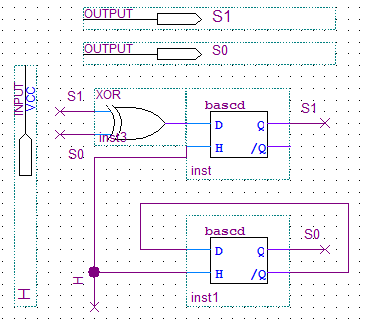
\includegraphics[scale=0.6]{inc3.PNG}\vspace{1em}
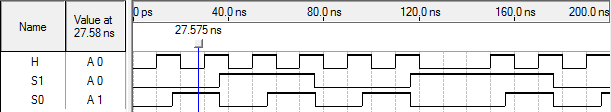
\includegraphics[scale=0.6]{sim1.PNG}
\caption{Incrémenteur sur 2 bits et simulation}
\label{inc3}
\end{figure}


\subsection*{Addition décimale de nombres à deux chiffres}

Le circuit Addec1 est immédiatement extensible aux nombres à deux chiffres puisqu'il suffit d'en disposer deux en reliant la retenue sortante des unités à l'entrante des dizaines, comme en Figure \ref{addec2}. On obtient alors un circuit combinatoire.

\clearpage

\begin{figure}[h]
\center
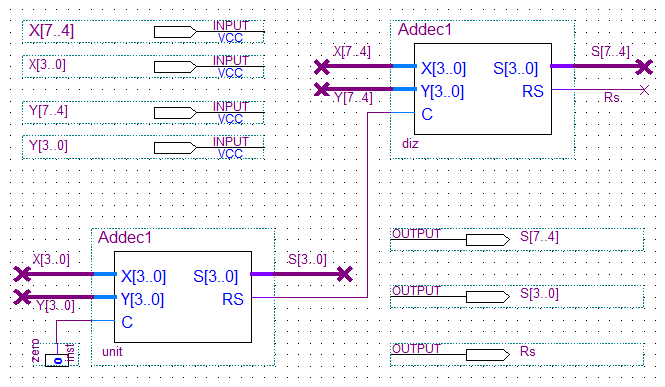
\includegraphics[scale=0.5]{addec2.PNG}
\caption{Additionneur de décimaux à deux chiffres}
\label{addec2}
\end{figure}

On souhaite utiliser une file de registres pour pouvoir entrer les chiffres un par un. On dispose en entrée du signal sur 4 bits correspondant au chiffre frappé, ainsi que d'un signal déclenché après la frappe ; il suffit alors d'enchaîner les registres à chargement systématique comme en Figure \ref{addec2total}.

\begin{figure}[h]
\center
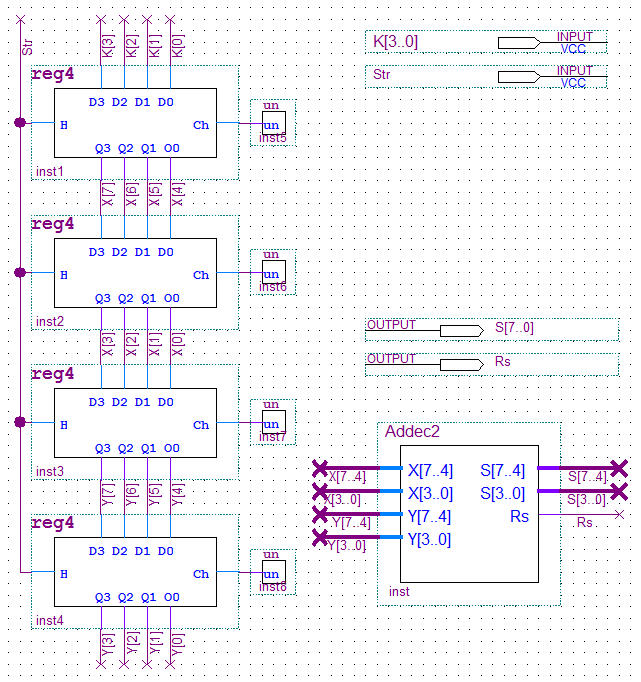
\includegraphics[scale=0.5]{addec2total.PNG}
\caption{Additionneur total}
\label{addec2total}
\end{figure}

\clearpage

\subsection*{Incrémenteur jusqu'à 5}

Pour un incrémenteur jusqu'à 5, il suffit de propager le signal d'incrément donné en entrée sur celui de l'incrémenteur 4 bits fourni sauf quand la sortie vaut 5, soit 0101. Ceci donne le circuit en Figure \ref{jqua5}.

\begin{figure}[h]
\center
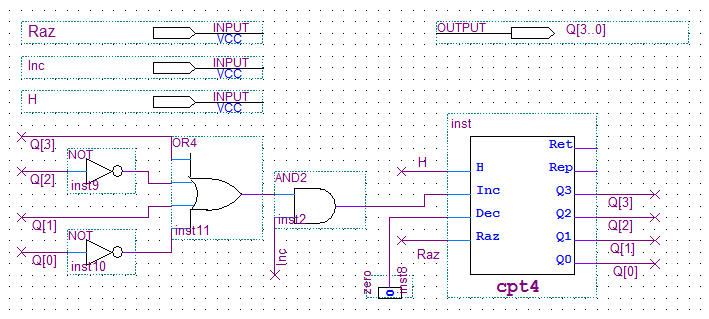
\includegraphics[scale=0.6]{jqua5.PNG}\vspace{1em}
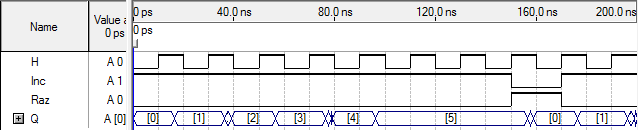
\includegraphics[scale=0.6]{sim3.PNG}
\caption{Schéma et simulation du circuit JQUA5}
\label{jqua5}
\end{figure}

\end{document}
